\documentclass[12pt,a4paper,fleqn]{article}

\usepackage{mystyle}

\begin{document}

	\begin{center}
		{\Huge
			\textbf{План работы в рамках курса\\
				по обучению основам\\
				параллельного программирования.\\
			}
		}
		\vspace{1em}
		{\large
			\textit{Дергачёв А.\,А., Ефимов О.\,В., Сметанина Е.\,О.\quad\textup{\textcopyleft}\\
				Московский государственный университет имени М.\,В. Ломоносова,\\
				Физический факультет, кафедра Общей физики и волновых процессов;\\
				Международный учебно-научный лазерный центр;\\
				НОЦ <<Суперкомпьютерные технологии>>\\
			}
		}
		\vspace{1em}
		\note{Версия 0.5beta1 от \today\\}
	\end{center}
	
	\vspace{0.5em}
\noindent \textbf{1. Введение и постановка задачи.}
\vspace{0.5em}

Нелинейное уравнение Шрёдингера играет существенную роль во многих областях физики, а также химии, экономики и иных наук.
Это уравнение на комплексную функцию $A(\vec{r},t)$ имеет вид:

\begin{equation}\label{NonlinearShredinger}
    \alpha i \dfrac{\partial A}{\partial t} = \beta \dfrac{\partial^2 A}{\partial x^2} + \gamma \left|A\right|^2 A
\end{equation}

Такое название присвоено уравнению (\ref{NonlinearShredinger}) потому, что его линейная часть совпадает с уравнением Шрёдингера.
В оптических приложениях чаще используется наименование <<нелинейное уравнение квазиоптики>>.

В нелинейной оптике это уравнение описывает самофокусировку  светового пучка в среде с кубической нелинейностью.
При описании распространения мощных коротких лазерных импульсов в диспергирующих средах
нелинейное уравнение для медленно меняющейся комплексной огибающей светового поля дополняют членами,
учитывающими дисперсию высших порядков, нелинейность отклика самоиндуцированной плазмы, потери на ионизацию и поглощение лазерного излучения в веществе \cite{KandidovShlenovKosarevaReview2009}.

В теории лазеров оптического диапазона с помощью нелинейного уравнения квазиоптики изучается усиление излучения, поиск собственных частот и типов колебаний поля в резонаторе.
Для исследования динамики усиленного спонтанного излучения в рентгеновском лазере используется квазиоптическое уравнение для поперечной корреляционной функции поля излучения \cite{LadaginStarikov1998}.

Распространение лазерных импульсов в оптических волноводах также описывается нелинейным уравнением квазиоптики для комплексной огибающей светового поля,
частными решениями которого являются темные (в области нормальной дисперсии групповых скоростей) и светлые (в области аномальной дисперсии групповых скоростей) солитоны \cite{Agrawal2001,Mahankov1983,VitkovskiyFedoruk2008}.

В физике сверхнизких температур нелинейное уравнение Шрёдингера используется для описания поведения неидеального бозе-газа со слабым взаимодействием между частицами \cite{Kadomcev1997}.
В работе \cite{Belyaeva2005} обращается внимание на математическую аналогию между теорией солитонных волн материи и теорией оптических солитонов в волоконных световодах.
Также нелинейное уравнение Шрёдингера используется в ядерной физике в рамках квантово-гидродинамической модели \cite{Kartvenko1993}, и, собственно, в гидродинамике для описания волн на поверхности жидкости \cite{Zeytunyan1995}.

В данной статье будет рассматриваться нелинейное уравнение квазиоптики в применении к задаче самофокусировки лазерного пучка.
Эффект самофокусировки возникает под действием изменения показателя преломления, вызванного Керровским эффектом.
В этом случае уравнение~(\ref{NonlinearShredinger}) с начальными условиями для гауссового пучка записывается в виде:
\begin{equation}\label{MainDim}
    \left\{
    \begin{array}{rcl}
        2ik\dfrac{\partial E}{\partial z} & = & \dfrac{\partial^2 E}{\partial x^2} + \dfrac{\partial^2 E}{\partial y^2} +
        \dfrac{2k^2}{n_0}n_2\left|E\left(x,y,z\right)\right|^2E\left(x,y,z\right)\\
        \\
        E(x,y,0) & = & E_0\exp\left\{-\dfrac{x^2+y^2}{2a_0^2}\right\},\quad (x,y)\in[-l,l]^2
    \end{array}
    \right.
\end{equation}

Здесь $E\left(x,y,z\right)$ "--- напряжённость электрического поля, $k$ "--- волновое число, $z$ "--- координата вдоль оси распространения светового пучка,
$x,y$ "--- координаты в поперечном сечении, $n_0$ и $n_2$ "--- линейный и нелинейный коэффициенты преломления.
В данном уравнении учтены такие физические факторы, как дифракция лазерного пучка и кубическая (по полю) нелинейность.

После обезразмеривания входящих в уравнение величин на их характерные значения $E=\tilde{E}\cdot E_0$, $x=\tilde{x}\cdot a_0$, $y=\tilde{y}\cdot a_0$, $z=\tilde{z}\cdot ka_0^2$ система будет выглядеть следующим образом:
\begin{equation}\label{MainNoDim}
    \left\{
    \begin{array}{rcl}
        2i\dfrac{\partial \tilde{E}}{\partial \tilde{z}} & = & \Delta_{\perp}\tilde{E} + R\left|\tilde{E}\right|^2\tilde{E}\\
        \\
        \tilde{E}(\tilde{x},\tilde{y},0) & = & \exp\left\{-\dfrac{\tilde{x}^2+\tilde{y}^2}{2}\right\}, \quad (x,y)\in\left[-\dfrac{l}{a_0},\dfrac{l}{a_0}\right]^2
    \end{array}
    \right.
\end{equation}


Здесь введены обозначения для поперечной части лапласиана $\Delta_{\perp}$ и коэффициента нелинейности $R$, которые будут использоватсья в дальшнейшем:
\begin{equation}
    \Delta_{\perp} = \dfrac{\partial^2}{\partial x^2} + \dfrac{\partial^2}{\partial y^2}
\end{equation}
\begin{equation}
    R = \dfrac{2k^2}{n_0} n_2 E_0^2 a_0^2
\end{equation}


\vspace{1em}
\noindent \textbf{2. Причины необходимости использования параллельных методов решения.}
\vspace{0.5em}

Основные проблемы численного моделирования задачи филаментации лазерных импульсов связаны с многомасшабностью задачи.
Поперечные масштабы пучка примерно на два порядка превосходят возникающие в нем структуры.
В то же время размер расчётной сетки должен на порядок превосходить радиус пучка, чтобы границы сетки не отсекали существенные части пучка,
а также чтобы иметь некоторую <<буферную область>>, в которую могла бы расширяться низкоинтенсивная периферийная часть пучка,
которая существенно влияет на распространение филамента \cite{KandidovShlenovKosarevaReview2009}.
В~противном случае также неизбежно возникновение краевых эффектов, приводящих к искажению решения.
На диаметр филамента должно приходиться достаточное количество точек (не менее 10), иначе резкие перепады интенсивности в окрестности филамента будут содержать слишком высокие пространственные частоты, что приведёт к невыполнению критерия Найквиста, наложению частот и, как следствие, неадекватности получаемого решения.
Как показывает практика, этот фактор является важным не только для метода решения, основанного на преобразовании Фурье, но и для остальных методов.

Таким образом, количество точек в поперечном сечении может достигать $10^4$ по каждой поперечной координате.
Рассматриваемая в статье задача не имеет временной зависимости, однако в реальных задачах филаментации рассматриваются короткие лазерные импульсы.
Для них количество временных слоев должно быть порядка $10^2-10^3$, а значит общее количество точек достигает величины порядка $10^{11}$,
а потребность в оперативной памяти "--- величины около 100~Гб.


\vspace{1em}
\noindent \textbf{3. Параллельные алгоритмы решения задачи.}
\vspace{0.5em}

Нами рассматриваются три метода численного решения уравнения (\ref{MainNoDim}).
Первый из них основан на использовании явной разностной схемы. Два других предусматривают предварительное расщепление по физическим факторам, при котором
интегрирование нелинейного уравнения квазиоптики сводится к последовательному интегрированию на каждом шаге интегрирования двух уравнений,
первое из которых описывает только дифракцию,а  второе "--- только нелинейность. Эти уравнения имеют следующий вид:
\begin{equation}\label{Split}
    \left\{
    \begin{array}{rcl}
        2i\dfrac{\partial E}{\partial z} & = & \Delta_{\perp}E \\
        \\
        2i\dfrac{\partial E}{\partial z} & = & R\left|E\right|^2E
    \end{array}
    \right.
\end{equation}

Если считать интенсивность поля ($I \sim |E|^2$) неизменной на протяжении одного шага нелинейности, что соблюдается при маленьких шагах по $z$,
то интегрирование уравнения для нелинейности не представляет проблем:
\begin{equation}\label{KerrSolution}
    E(x,y,z_i + \Delta z) = E(x,y,z_i)\exp\left(-\frac{iR}{2}\left|E(x,y,z_i)\right|^2\Delta z\right)
\end{equation}

Отметим, что поскольку нелинейность является локальной, то есть набег фазы
в точке поперечного сечения зависит только от значения интенсивности поля в этой же точке,
то для решения второго уравнения из системы (\ref{Split}) можно успешно применить метод геометрического параллелизма,
который будет иметь идеальную масштабируемость при любом количестве используемых для вычислений процессоров.

Для интегрирования уравнения дифракции в случае расщепления по физическим факторам были использованы два метода:
метод на основе неявной разностной схемы и метод, использующий быстрое преобразование Фурье.


	\section{Явная схема.}
\begin{multline*}
	2i\frac{\partial E}{\partial z}=\triangle_\perp E + R\left|E\right|^2E \\
	{\hbox to 0.7cm{\rightarrowfill}}\quad
	E_{i,j}^{(n+1)}=E_{i,j}^{(n)}+\frac{\Delta z}{2i}
	\left(\frac{E_{i,j+1}^{(n)} + E_{i,j-1}^{(n)} + E_{i+1,j}^{(n)} + E_{i-1,j}^{(n)} - 
	4E_{i,j}^{(n)}}{\Delta x^2} + R\left|E_{ij,}^{(n)}\right|^2E_{i,j}^{(n)}
	\right)
\end{multline*}

\begin{itemize}
	\item  Не используя метод расщепления по физическим факторам, реализовать приведенную 
		выше явную схему.
	\item Для численного интегрирования уравнения использовать метод Рунге-Кутта четвертого
		порядка точности.
	\item Использовать блочное распределение матрицы между процессами.
\end{itemize}


	\section{Метод Фурье.}


\subsection{Освоение \fftw.}

\begin{itemize}
	\item Разобраться с подключением {\fftw} в проект Visual Studio. Мануал по {\fftw} 2.1.3 есть на сайте \href{http://fftw.org}{fftw.org}.
	\item Разобраться с распределением матрицы между процессами, необходимым для \fftw.
	\item Разобраться с расположением результата одного фурье-преобразования и нормировкой.
	\item Реализовать \code{fftw\_mpi(...)} туда-обратно при гауссовых начальных условиях в двумерном случае.
\end{itemize}


\subsection{Дифракция в линейной среде.}
\begin{multline*}
	\left\{
	\begin{array}{rcl}
		2i\dfrac{\partial E}{\partial{z}}&=&\dfrac{\partial^2 E}{\partial{x^2}}+
		\dfrac{\partial^2 E}{\partial{y^2}}\\
		E(x,y,0)&=&\exp\left\{-\dfrac{x^2+y^2}{2}\right\},\quad (x,y)\in[-l,l]^2
	\end{array}
	\right.
	\quad{\hbox to 0.7cm{\rightarrowfill}}\\
	{\hbox to 0.7cm{\rightarrowfill}}\quad
	\Biggl[
	E(x,y,z)=\sum\limits_{j,k}\tilde{E}_{jk}(z)\exp\left\{\dfrac{2\pi ijx}{N}\right\}
	\exp\left\{\dfrac{2\pi iky}{N}\right\}
	\Biggr]
	\quad{\hbox to 0.7cm{\rightarrowfill}}\\
	{\hbox to 0.7cm{\rightarrowfill}}\quad
	\left\{
	\begin{array}{rcl}
		2i\dfrac{\partial\tilde E}{\partial{z}}&=&\left(\dfrac{2\pi i}{N}\right)^2(j^2+k^2)
		\tilde E(z)\\
		\tilde E_{jk}(0)&=&\tilde E^{(0)}
	\end{array}
	\right.
	\quad{\hbox to 0.7cm{\rightarrowfill}}\\
	{\hbox to 0.7cm{\rightarrowfill}}\quad
	\tilde E_{jk}(z)=\tilde E^{(0)}\exp\left\{i\dfrac{2\pi^2}{N^2}(j^2+k^2)z\right\}
\end{multline*}

\begin{multline*}
	\text{Итого:}\hspace{0.5cm}E(x,y,0)
	\hspace{0.5cm}{\buildrel\hbox{2D FFT}\over{\hbox to 2cm{\rightarrowfill}}}
	\hspace{0.5cm}\tilde E_{jk}(0)
	\hspace{0.5cm}\hbox to 1cm{\rightarrowfill}\\
	\hbox to 1cm{\rightarrowfill}
	\hspace{0.5cm}\tilde E_{jk}(0)\exp\left\{i\dfrac{2\pi^2}{N^2}(j^2+k^2)z\right\}
	\hspace{0.5cm}{\buildrel{\hbox{2D FFT}^{-1}}\over{\hbox to 2cm{\rightarrowfill}}}
	\hspace{0.5cm}E(x,y,z)
\end{multline*}

\begin{itemize}
	\item Реализовать параллельный расчет дифракции гауссового пучка.
        \item Сравнить с аналитическим решением.
        \item Исследовать зависимость времени счёта от следующих параметров:
		\begin{itemize}
			\item с буфером и без него;
			\item \code{FFTW\_NORMAL\_ORDER} vs \code{FFTW\_TRANSPOSED\_ORDER};
			\item (опционально) \code{FFTW\_ESTIMATE} vs \code{FFTW\_MEASURE};
			\item (опционально) \code{wisdom}, OpenMP, ...
		\end{itemize}
	\item Выбрать оптимальные параметры для использования в следующем пункте.
\end{itemize}


\subsection{Дифракция в нелинейной среде.}
\begin{equation*}
	\left\{
	\begin{array}{rcl}
		2i\dfrac{\partial E}{\partial z}&=&R\left|E\right|^2E\\
		E(x,y,0)&=&E_0(x,y)
	\end{array}
	\right.
	\rightarrow
	E(x,y,z)=E_0(x,y)\exp\left\{-i\dfrac{R\left|E_0(x,y)\right|^2}{2}z\right\}
\end{equation*}

\begin{itemize}
	\item Выполнять шаг дифракции и шаг нелинейности в разном порядке:
	\begin{enumerate}
		\item <<дифракция "--- нелинейность>>
		\item <<нелинейность "--- дифракция>>
		\item чередовать
	\end{enumerate}
	\item Изменять шаг интегрирования для выполнения условия $\Delta\varphi_{\text{нл}}=\dfrac{R\left|E_{max}\right|^2}{2}\Delta z < 0.1$.
	\item Использовать оптимальные параметры \fftw, найденные в предыдущем пункте.
	\item Получить формулу Марбургера для гауссова пучка и ее аналог для $\ch^{-1}$ пучка.
\end{itemize}


	\subsection{Метод с использование неявной схемы}
Используемая консервативная разностная схема для исходного уравнения (\ref{MainNoDim}) для неравномерных сеток в поперечном сечении была предложена в (\cite{SweepScheme}). Она выглядит следующим образом:

\begin{equation}\label{sweep_diff_sys}
    \left\{
    \begin{aligned}
        2i\frac{h_1}{2}\frac{\hat{E}_{0,j}-E^k_{0,j}}{\Delta z} &= \frac{1}{2}\left(\frac{\hat{E}_{1,j}-\hat{E}_{0,j}}{h_1}\right) + \frac{1}{2}\left(\frac{E^k_{1,j}-E^k_{0,j}}{h_0}\right)\\
        2i\frac{h_{i+1}+h_i}{2}\frac{\hat{E}_{i,j}-E^k_{i,j}}{\Delta z} &= \frac{1}{2}\left(\frac{\hat{E}_{i+1,j}}{h_{i+1}} -\left(\frac{1}{h_{i+1}} + \frac{1}{h_i}\right)\hat{E}_{i,j} + \frac{\hat{E}_{i-1,j}}{h_i}\right) \\
        &\qquad+ \frac{1}{2}\left(\frac{E^k_{i+1,j}}{h_{i+1}} -\left(\frac{1}{h_{i+1}} + \frac{1}{h_i}\right)E^k_{i,j} + \frac{E^k_{i-1,j}}{h_i}\right),\quad i=1,\ldots N\\
        2i\frac{h_N}{2}\frac{\hat{E}_{N,j}-E^k_{N,j}}{\Delta z} &= \frac{1}{2}\left(\frac{\hat{E}_{N,j}-\hat{E}_{N-1,j}}{h_N}\right) + \frac{1}{2}\left(\frac{E^k_{N,j}-E^k_{N,j}}{h_{N-1}}\right)
    \end{aligned}
    \right.
\end{equation}

Указанная схема осуществляет расчет <<дифракции по $x$>>.
Аналогичная система разностных уравнений рассчитывает <<дифракцию по $y$>>.
Если шаг сетки равномерный, то есть $h_i=x_i-x_{i-1}=const$, то схема переходит в хорошо известную схему Кранка-Николсона.
Учет керровской нелинейности осуществляется в рамках описан в разделе \ref{SplitMethod}.

Указанная система является системой относительно значений поля на промежуточном слое $\hat{E}_{i,j}$.
Матрица системы трехдиагональна и решается методом прогонки (ссылка на Калиткина).
Рассмотрим вариант параллельной реализации прогонки.

\begin{figure}[h]
    \begin{center}
        \begin{minipage}{0.48\linewidth}
            \center{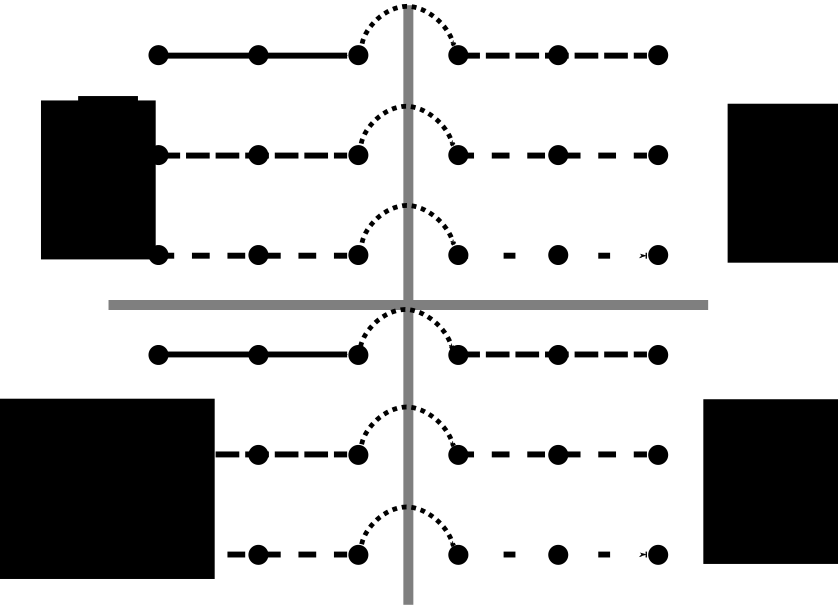
\includegraphics[width=0.95\linewidth]{\imagesdir/sweep_method_forward.png}} \\
            \caption{Метод с использованием неявной схемы. Прямая прогонка.}
            \label{img:sweepforward}
        \end{minipage}
        \hfill
        \begin{minipage}{0.48\linewidth}
            \center{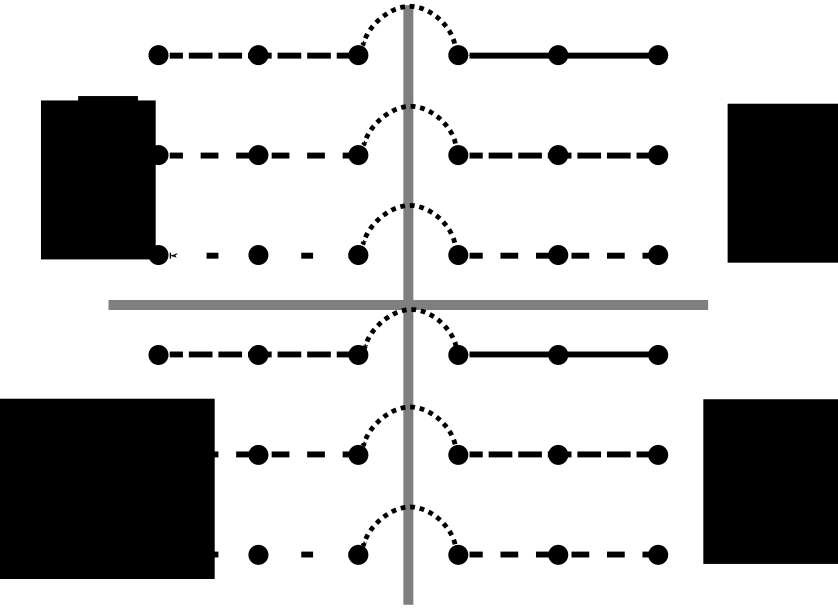
\includegraphics[width=0.95\linewidth]{\imagesdir/sweep_method_backward.png}} \\
            \caption{Метод с использованием неявной схемы. Обратная прогонка.}
            \label{img:sweepbackward}
        \end{minipage}
    \end{center}
\end{figure}

На рис. \ref{img:sweepforward}, \ref{img:sweepbackward} черными точками изображены точки расчетной сетки.
Вертикальная и горизонтальная светло-серые прямые показывают разбиение матрицы поперечного сечения между процессами.
Римские цифры обозначают номера процессов.
Цветные стрелки соответствуют вычислению прогоночных коэффициентов.
Серые стрелки отображают обмены данными между процессами.

Первому расчетному шагу соответствуют стрелки красного цвета.
Для цикла прямой прогонки их выполняют процессы первого столбца матрицы процессов.
Далее эти процессы пересылают посчитанные коэффициенты в граничной точке соседнему справа процессу.
Следующий такт отображен стрелками зеленого цвета, далее следуют синие и коричневые стрелки.
Таким образом, по каждой строке матрицы процессов запускается конвейерная схема параллельных вычислений.

В цикле обратной прогонки конвейерная схема запускается в обратную сторону (соответствие цвета стрелок и порядка выполнения расчетных операций то же).
Пересылке теперь подвергаются расчитанные значения поля.

Отметим две особенности метода.
Во-первых, поскольку цикл обратной прогонки запускается после окончания прямой прогонки по всем строкам расчетной сетки, то необходимо хранить в памяти прогоночные коэффициенты для всех строк, то есть необходима дополнительная матрица для прогоночных коэффициентов того же размера, что и матрица поля.
Во-вторых, для расчета коэффициентов, фигурирующих в разностной системе (\ref{sweep_diff_sys}), необходим обмен значениями поля в граничных областях.

Отметим также, что для высокой эффективности параллельного алгоритма необходимо, чтобы количество строк матрицы поля у отдельного процесса было существенно больше количества процессов в строке матрицы процессов.
Действительно, если число строк у отдельного процесса равно $N_{loc}$, а число процессов в строке матрицы процессов равно $q$ (на рис. \ref{img:sweepforward}, \ref{img:sweepbackward} $N_{loc}=3$, $q=2$), то на цикл прямой прогонки потребуется $N_{loc}+q$ итераций.
Таким образом, верхняя оценка на эффективность имеет вид:
\begin{equation}
    E_n\leqslant\frac{N_{loc}q^2}{q^2(N_{loc} + q)}=\frac{1}{1+q/N_{loc}}.
\end{equation}

В этом соотношении не учтены потери времени на пересылки и синхронизацию процессов. 
	\section{Входные параметры и формат выходных файлов.}
\label{sec:detailed_description}


\subsection{Начальные условия.}
Начальное распределение должно иметь вид гауссова пучка. Размер счётной области -- 10 радиусов пучкая.
Сгенерировать такое распределение можно с помощью \href{http://github.com/Sannis/create_2d_func/}{create\_2d\_func}
(\href{http://github.com/Sannis/create_2d_func/tarball/v1.0}{стабильная версия 1.0}) со следующими аргументами:
\begin{verbatim}
$> mpirun -np 8 ./create_2d_func -n 1024 -f gauss \
       -l 5 --a0 1 --r0 1 ./gauss_n1024_l5.cpl
\end{verbatim}


\subsection{Проводимые расчёты.}
\begin{enumerate}
	\item Время выполнения одного шага дифракции с использованием различных флагов \fftw. Параметры:
		\begin{itemize}
			\item $N = 1024, 8192$.
			\item $np = 1, 8, 32$ для СКИФ <<Чебышёв>> \\ и $np = 128, 1024$ для IBM Bluegene/P.
		\end{itemize}
		Сравнить скорость работы {\fftw} при использовании дополнительного буфера и без него,
		степень зависимости времени выполнения от использования флагов \\ FFTW\_NORMAL\_ORDER и FFTW\_TRANSPOSED\_ORDER.
	\item Время расчёта распространения пучка в нелинейной среде на одну дифракционную длину(до $z=1$). Параметры:
		\begin{itemize}
			\item $R = 5,\text{ }\Delta\varphi < 0.1$.
			\item $N = 512, 1024, 2048, 4096, 8192, 16384, 32768$.
			\item $np = 1, 2, 4, 8, 16, 32, 64, 128$ для СКИФ <<Чебышёв>> \\ и $np = 128, 256, 512, 1024$ для IBM Bluegene/P.
		\end{itemize}
		Провести замер времени выполнения расчётной части программы в друх вариантах:
		только распространение и распространение с сохранением результируещего поля и максимальной интенсивности пучка каждые 10 шагов.
		После расчёта с сохранением бинарные данные можно удалить или использовать для оценки точности метода, чтобы сократить
		число запусков программы. Столбец полной можности пучка в выходной таблице можно заполнить нулями.
		
	\item Точность алгоритмов для случая линейного распространения на одну дифракционную длину(до $z=1$). Параметры:
		\begin{itemize}
			\item $R = 0$.
			\item $N = 512, 2048, 8192$.
			\item $\Delta z = 0.001$, соответственно 1000 шагов.
		\end{itemize}
		Результатом работы программы должна быть таблица с данными об изменении максимальной интенсивности
		и полной мощности пучка при распространении. Формат таблицы будет приведён ниже.
		Также необходимо сохранить в файл конечное распределение поля при $z=1$.
	
	\item Точность алгоритмов для случая нелинейного распространения на одну дифракционную длину(до $z=1$). Параметры:
		\begin{itemize}
			\item $R = 5,\text{ }\Delta\varphi < 0.1$.
			\item $N = 512, 2048, 8192$.
		\end{itemize}
		Результатом работы программы должна быть таблица с данными об изменении максимальной интенсивности
		и полной мощности пучка при распространении. Формат таблицы будет приведён ниже.
		Также необходимо сохранить в файл конечное распределение поля при $z=1$.
\end{enumerate}


\subsection{Правила именования файлов и папок с результатами.}
Результаты должны располагаться в папках следующего вида(относительно папки запускаемой программы):
\begin{itemize}
	\item Для сравнения скорости работы {\fftw} с разными флагами: \\
		\texttt{./results/Skif/FFTW\_compare/(no|with)buffer\_(no|with)transpose/N1024\_NP16=4x4/}
	\item Для замеров времени без сохранения: \\
		\texttt{./results/Skif/Time\_no\_save/N1024\_NP16=4x4/}
	\item Для замеров времени c сохранением: \\
		\texttt{./results/Skif/Time\_with\_save/N1024\_NP16=4x4/}
	\item Для оценки точности: \\
		\texttt{./results/Skif/Accuracy\_r0/N1024\_NP16=4x4/} и \\
		\texttt{./results/Skif/Accuracy\_r5/N1024\_NP16=4x4/}
\end{itemize}
В каждой папке должен располагаться файл log.txt с входными данными и результатами работы программы. Бинарные файлы с распределением поля на отдельных шагах должны располагаться в файлах вида out\_00070.cpl. Распределение поля в конце трассы (при $z=1$) должно быть сохранено под именем out\_z1.cpl.


\subsection{Формат выходного лога программы.}
В начале вывода программы должны присутствовать значения параметров сетки и расчётных параметров.
Далее должна следовать таблица, содержащая колонки со значениями текущего шага, координаты, максимальной интенсивности и полной мощности пучка. В последней строке нужно вывести время выполнения расчётной части программы. \\
Образец:
\begin{verbatim}
    =========================================
    === Propagation: Diffraction and Kerr ===
    =========================================

MPI grid size: 1 (1x1)

N: 256
L: 5.000000
Impulse file: ../../data/gauss_n256_l5.cpl

R: 0.000000
dz: 0.001000 (dphi < 0.1)
Steps: 1000

n        dz          z           I_max(z)          P(z)
00000    0.010000    0.000000    1.000000000000    0.999999999997
00001    0.010000    0.010000    0.999900162406    0.999999999997
00002    0.010000    0.020000    0.999600769015    0.999999999997

...

Execution time(sec):
144.044038
\end{verbatim}


\subsection{Обработка результатов.}
\begin{itemize}
	\item Для оценки точности алгоритмов необходимо произвести сравнение формы импульсов после распространения на одинаковую длину.
		В случае линейного распространения результат работы каждого алгоритма можно сравнить с аналитическим решением,
		в случае нелинейного --- только между собой. Для сравнения используется программа \href{http://github.com/Sannis/bindiff/}{bindiff}
(\href{http://github.com/Sannis/bindiff/tarball/v1.0}{стабильная версия 0.1}).
		
	\item Построение графиков осуществить в автоматическом режиме с использованием bash скриптов и \href{http://www.gnuplot.info/}{gnuplot}.
	
	\item Визуализировать бинарные данные можно с использованием программы \href{http://github.com/Sannis/bin2gif/}{bin2gif}
(\href{http://github.com/Sannis/bin2gif/tarball/v0.3}{стабильная версия 0.3}).
\end{itemize}


\subsection{Отчётные данные.}

\begin{itemize}
	\item Времена работы алгоритма {\fftw} при различных параметрах. Выбранные оптимальные параметры.
	\item Времена работы всех перечисленных алгоритмов без сохранения и с учётом сохранения. Ускорение работы программ в зависимости от количества процессов.
	\item Интегральная среднеквадратичная ошибка в распределении поля при дифракции гауссова пучка (линейный случай).
	\item \ZZZ{Интегральная среднеквадратичная ошибка в соответствии с формулой Марбургера для расстояния филаментации (нелинейный случай).}
\end{itemize}

	\section{Исполнители.}
\label{sec:authors}

Дергачёв А.\,А. <\href{mailto:dergachev88@yandex.ru}{dergachev88@yandex.ru}>:
Метод прогонки. \par
Ефимов О.\,В. <\href{mailto:efimovov@yandex.ru}{efimovov@yandex.ru}>:
Метод Рунге-Кутта \par
Сметанина Е.\,О. <\href{mailto:jannes-2002@yandex.ru}{jannes-2002@yandex.ru}>:
Метод БПФ.

\end{document}

